\section{Formal Grammars}
\subsection{Defining a Language}
Now we introduce formal grammars as a way of building up our language.
This is similar to English, where we have a grammar system that tells us how to build sentences.
For example, we know the basic structure of a sentence is \textit{subject-verb-object}. \\

\noindent
We can write \textbf{linear} statements such as ``John hit the ball'', which has an underlying \textbf{hierarchical} structure that permits it:

\begin{figure}[h]
\centering
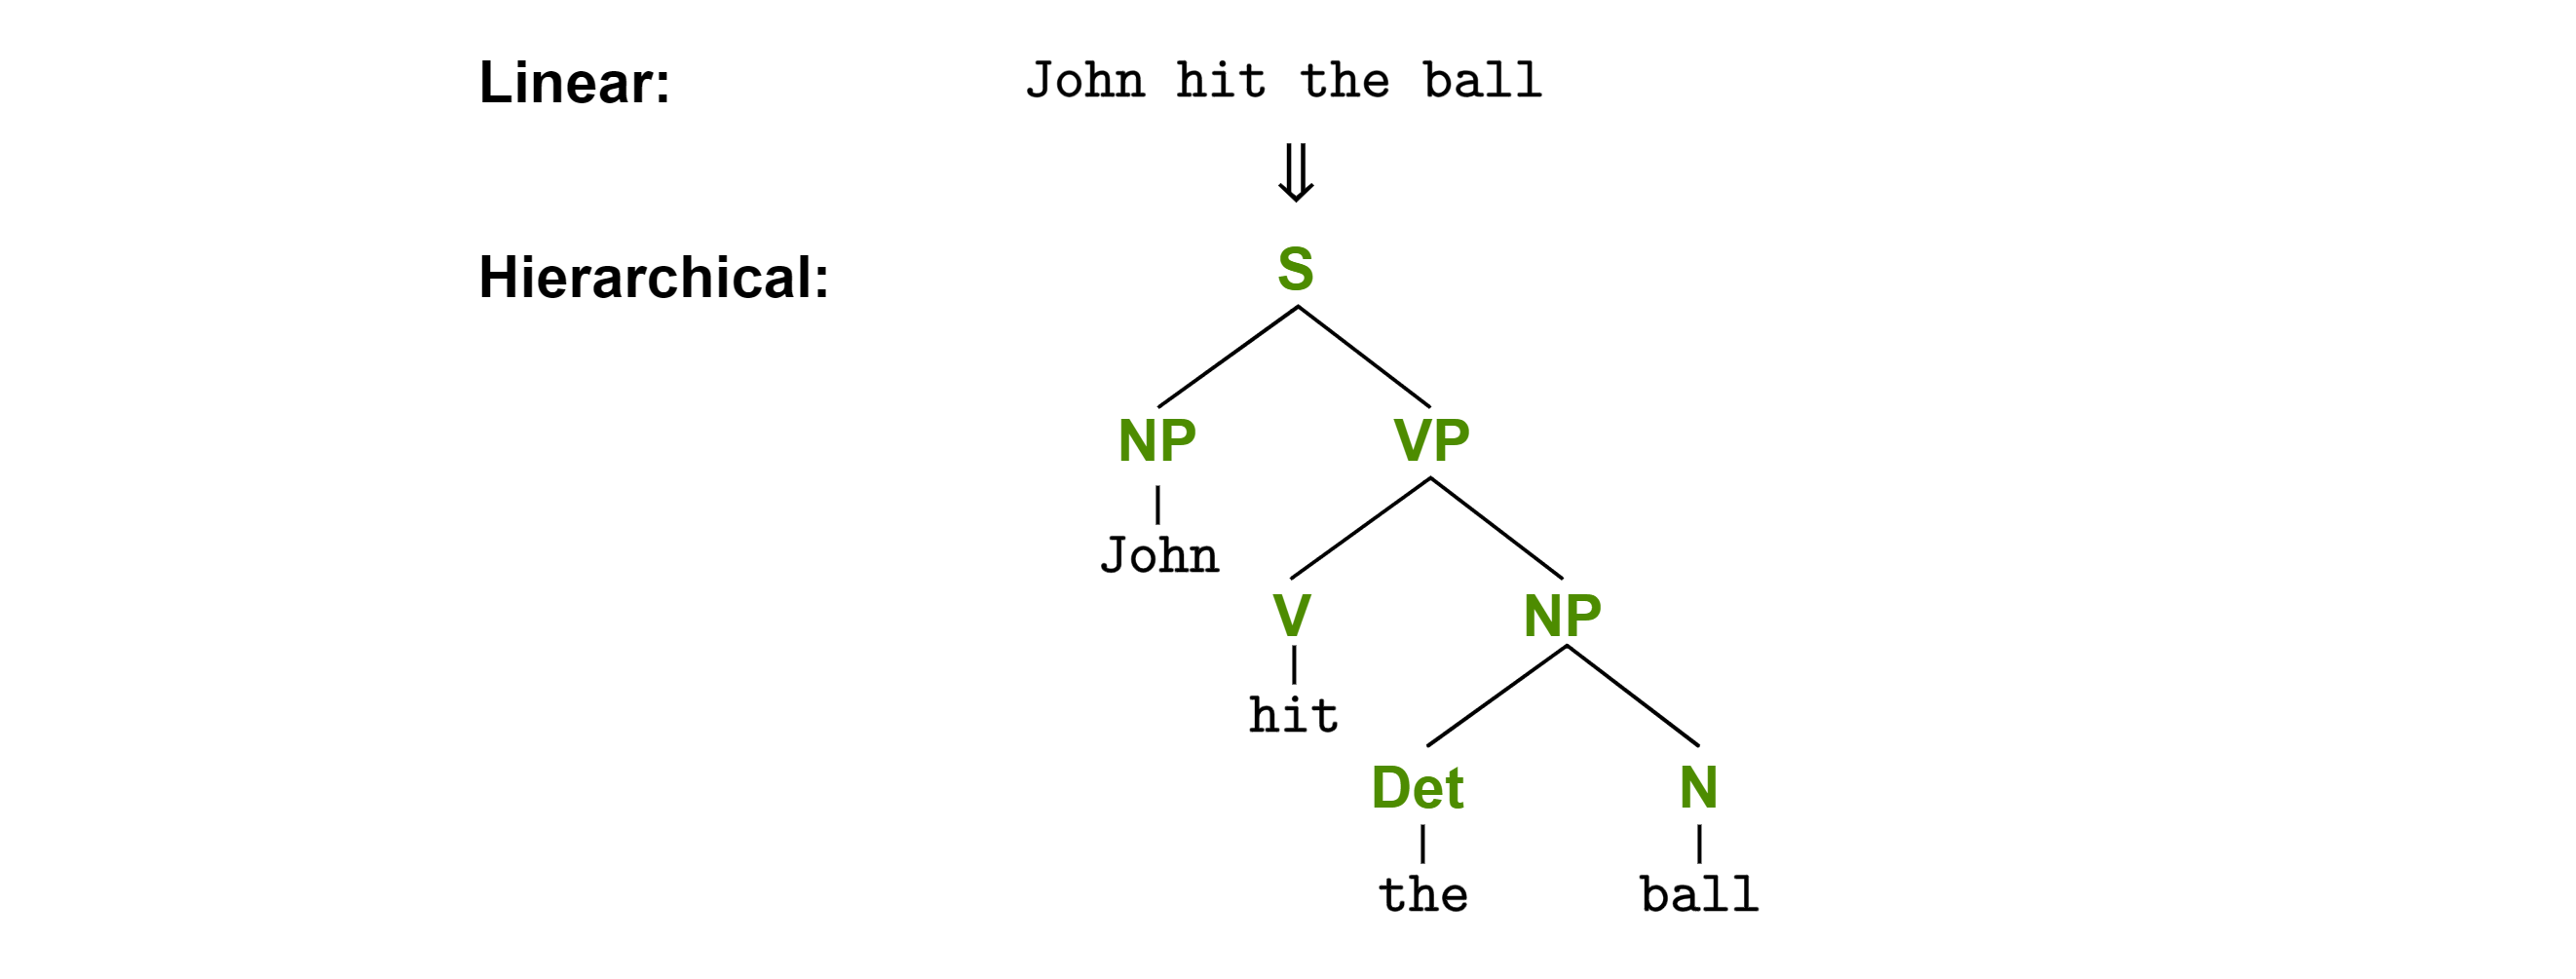
\includegraphics[width=1\textwidth]{Sections/Formal/eng.png}
\caption{The sentence ``John hit the ball'' has an underlying hierarchical structure of a tree. Here, \textbf{S}: Sentence (the root of the tree), \textbf{NP}: Noun Phrase (a phrase centered around a noun), \textbf{VP}: Verb Phrase (a phrase centered around a verb), \textbf{V}: Verb (the action in the sentence), \textbf{Det}: Determiner (words like "the", "a", "an", which specify nouns), and \textbf{N}: Noun (person, place, thing, or idea).}
\end{figure}

\noindent
\textbf{Grammar vs. Semantics:} Notice the english sentence 

\begin{center}
\Large \textit{``Your air tied a toothbrush at school!''}
\end{center}

\noindent
is grammatically correct, but carries little to no meaning. In contrast, 
the sentence

\begin{center}
\Large \textit{``Colorless the of allegator run am sleepily''}
\end{center}

\noindent
is perhaps an unsettling read, as it is not grammatically correct. \\

\newpage 

\noindent
The same way we can represent english sentences in a tree structure, is the same way we can represent programs. First 
we define the difference between an \textbf{interpreter} and a \textbf{compiler}.

\begin{Def}[Interpreter]

    An \textbf{interpreter} is a program that directly executes instructions written in a programming language without 
    requiring a machine code translation. The typical stages are:
    
    \begin{enumerate}
        \item \textbf{Lexical Analysis}: Reads a string of characters (program), converting it into tokens.
        \item \textbf{Syntax Analysis}: Parses these tokens to build an abstract syntax tree (AST).
        \item \textbf{Semantic Analysis}: Checks for semantic errors and annotates the AST.
        \item \textbf{Intermediate Representation (IR) Generation}: Converts the AST into an intermediate representation (IR) to facilitate execution.
        \item \textbf{Direct Execution}: Executes the IR or AST directly using an interpreter.
    \end{enumerate}
    
    \noindent
    Interpreted languages are \textbf{evaluated at runtime} (e.g., Python, Ruby, JavaScript). Some interpreters use an \textbf{AST-based execution}, while others generate an \textbf{IR} (e.g., Python's bytecode for the CPython interpreter).
    
    \end{Def}
    
    \begin{Def}[Compiler]
    
    A \textbf{compiler} is a program that translates code written in a high-level programming language into a lower-level language, typically machine code, to create an executable program. This involves several stages:
    
    \begin{enumerate}
        \item \textbf{Lexical Analysis}: Reads the source code and converts it into tokens.
        \item \textbf{Syntax Analysis}: Parses these tokens to construct an abstract syntax tree (AST).
        \item \textbf{Semantic Analysis}: Validates the AST against language rules and performs type checking.
        \item \textbf{Intermediate Representation (IR) Generation}: Transforms the AST into a lower-level representation that is easier to optimize and translate.
        \item \textbf{Optimization}: Enhances the IR to improve performance and efficiency.
        \item \textbf{Code Generation}: Translates the optimized IR into machine code or another target language.
    \end{enumerate}
    
    \noindent
    Compiled languages are \textbf{translated before runtime} (e.g., C, C++, Rust, OCaml). The \textbf{IR} plays a crucial role in optimizing the compilation process, as seen in LLVM or Java’s bytecode execution in the JVM.
    
    \end{Def}
   
\newpage 

\noindent
The following diagram illustrate the translation process of a compiler and an interpreter:

\vspace{2em}

\begin{figure}[h]
    \hspace{-2em}
    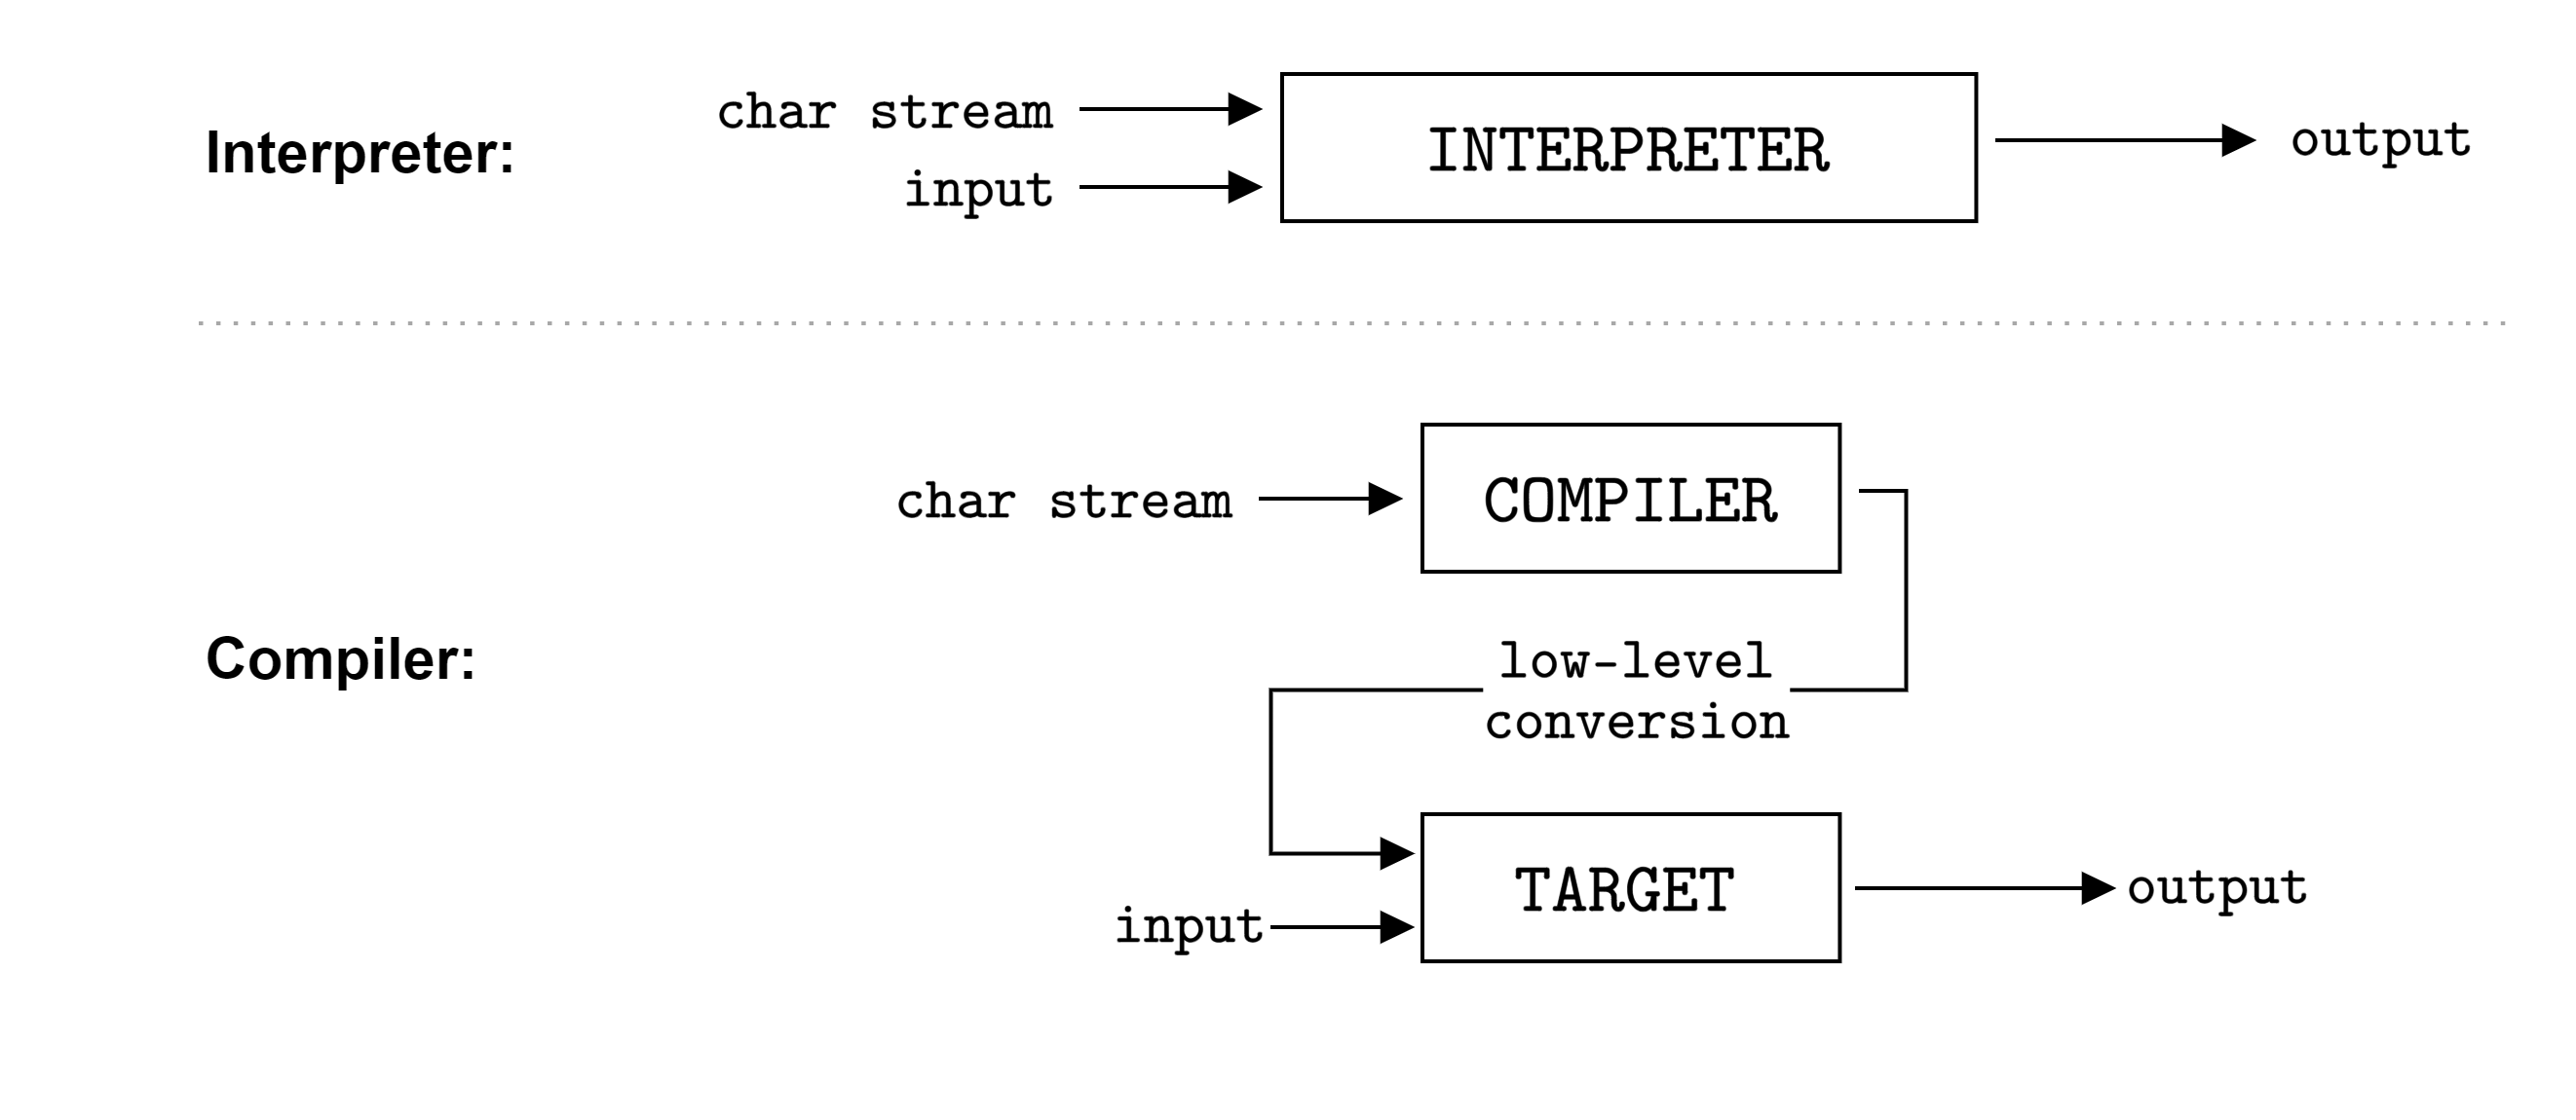
\includegraphics[width=1\textwidth]{Sections/Formal/comp.png}
    \caption{The high-level processes of a compiler and an interpreter.}
\end{figure}

\begin{figure}[h]
    \centering
    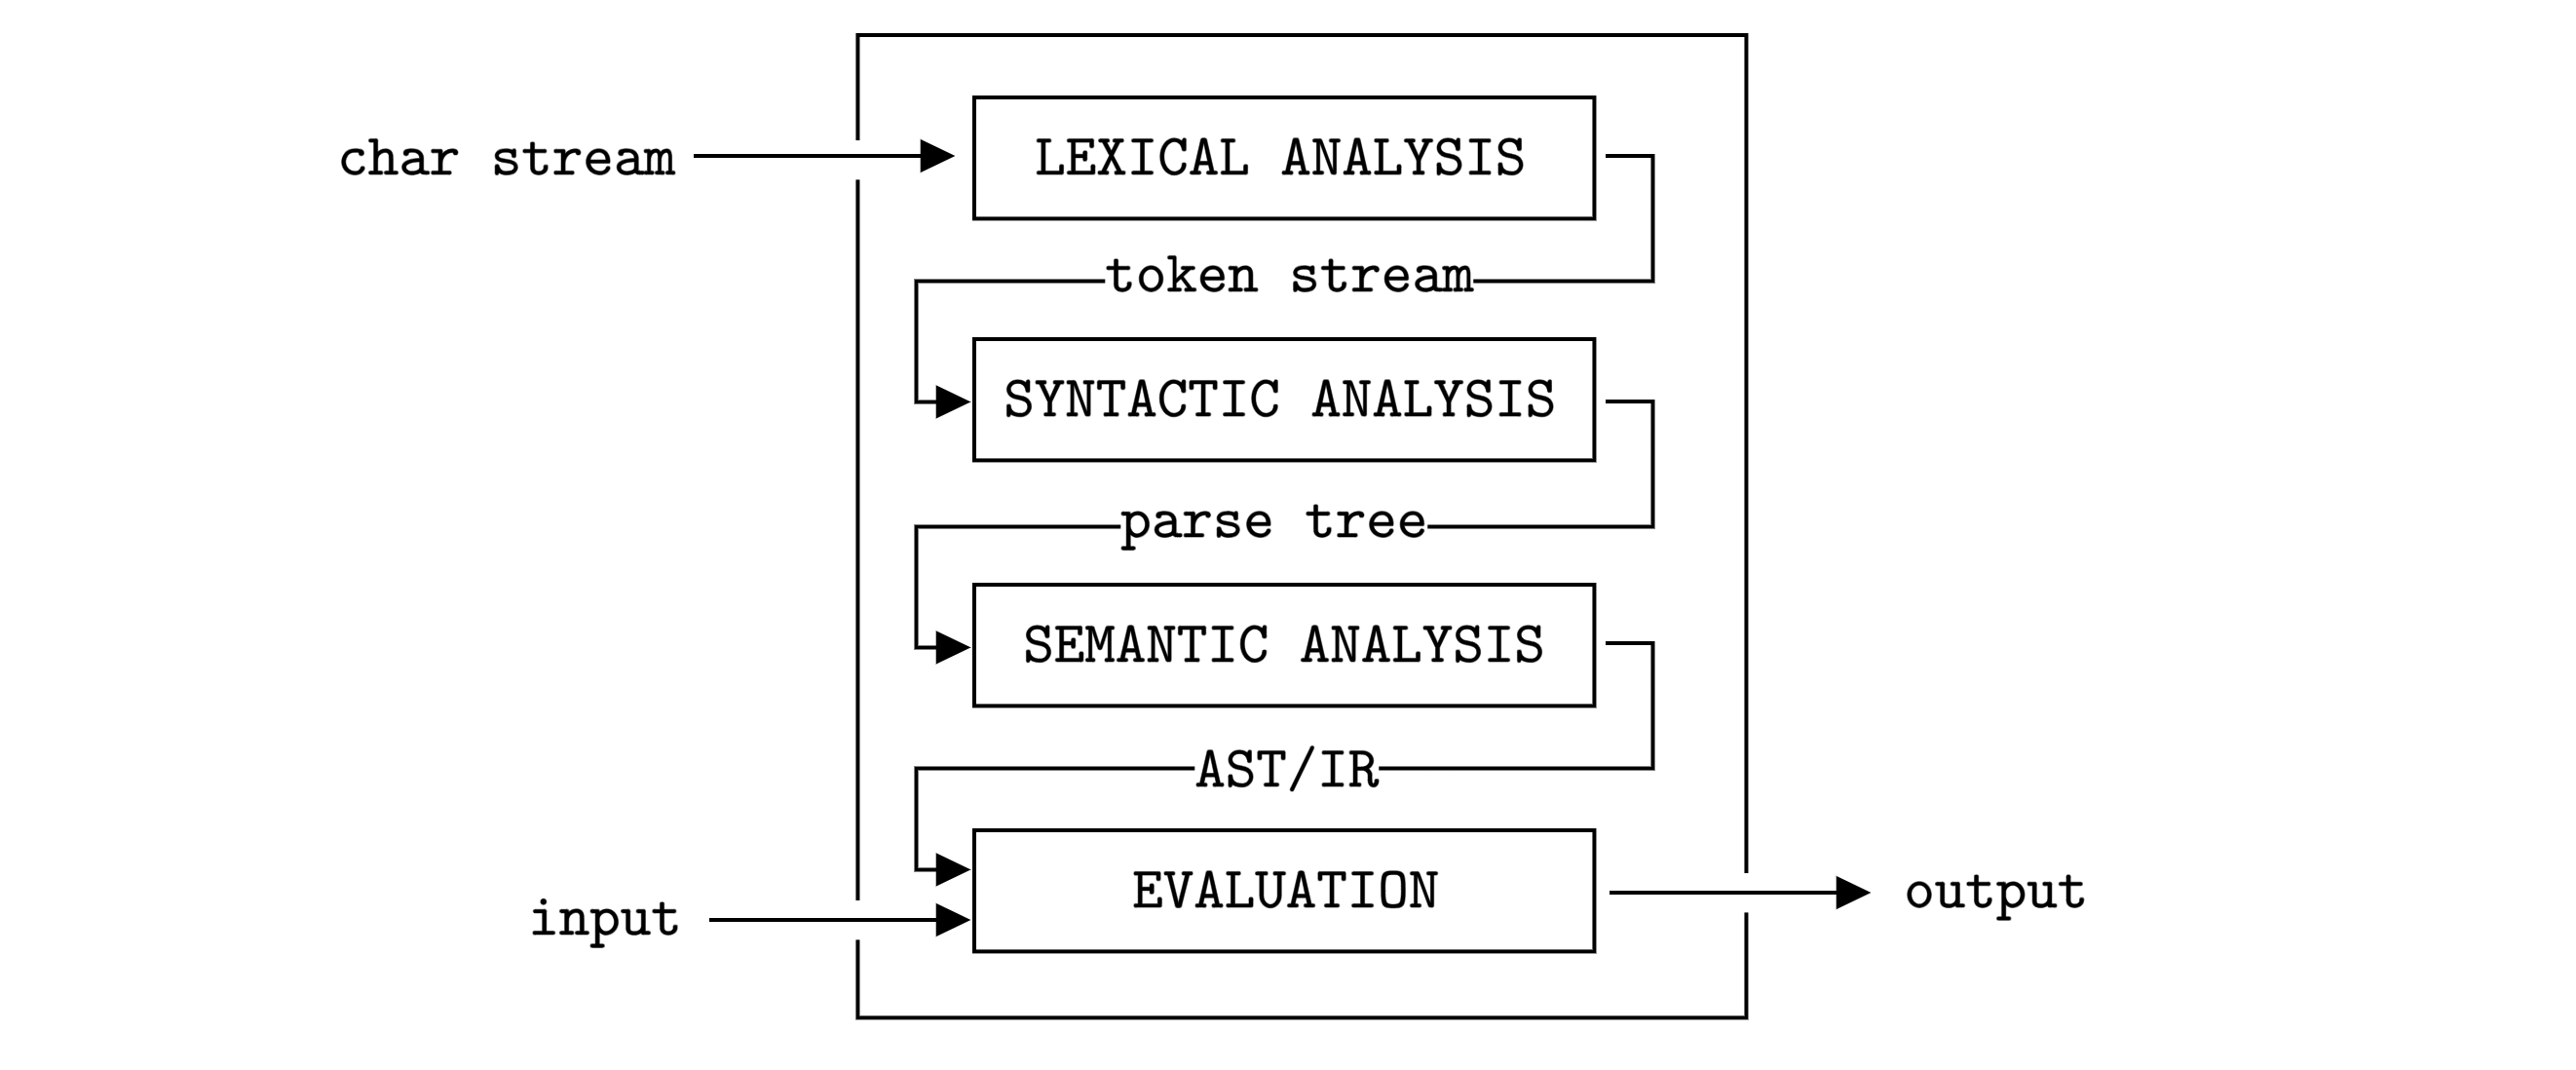
\includegraphics[width=1\textwidth]{Sections/Formal/comp2.png}
    \caption{Stages of program processing: A character stream undergoes lexical, syntactic, and semantic analysis, transforming into an AST or IR before evaluation. Interpreters execute the AST/IR directly, while compilers translate it into machine code.}
\end{figure}

\newpage
    
\noindent
\noindent
To formally layout our language, we use the \textbf{Backus-Naur Form (BNF)} notation. But before we 
do so, we gain some intuition by breaking down an english sentence from its \textbf{terminal symbols} to its \textbf{non-terminal symbols}. Recall these terms from the pre-requisite section (\ref{def:non-terminal-terminal}).\\

\begin{figure}[h]
    \centering
    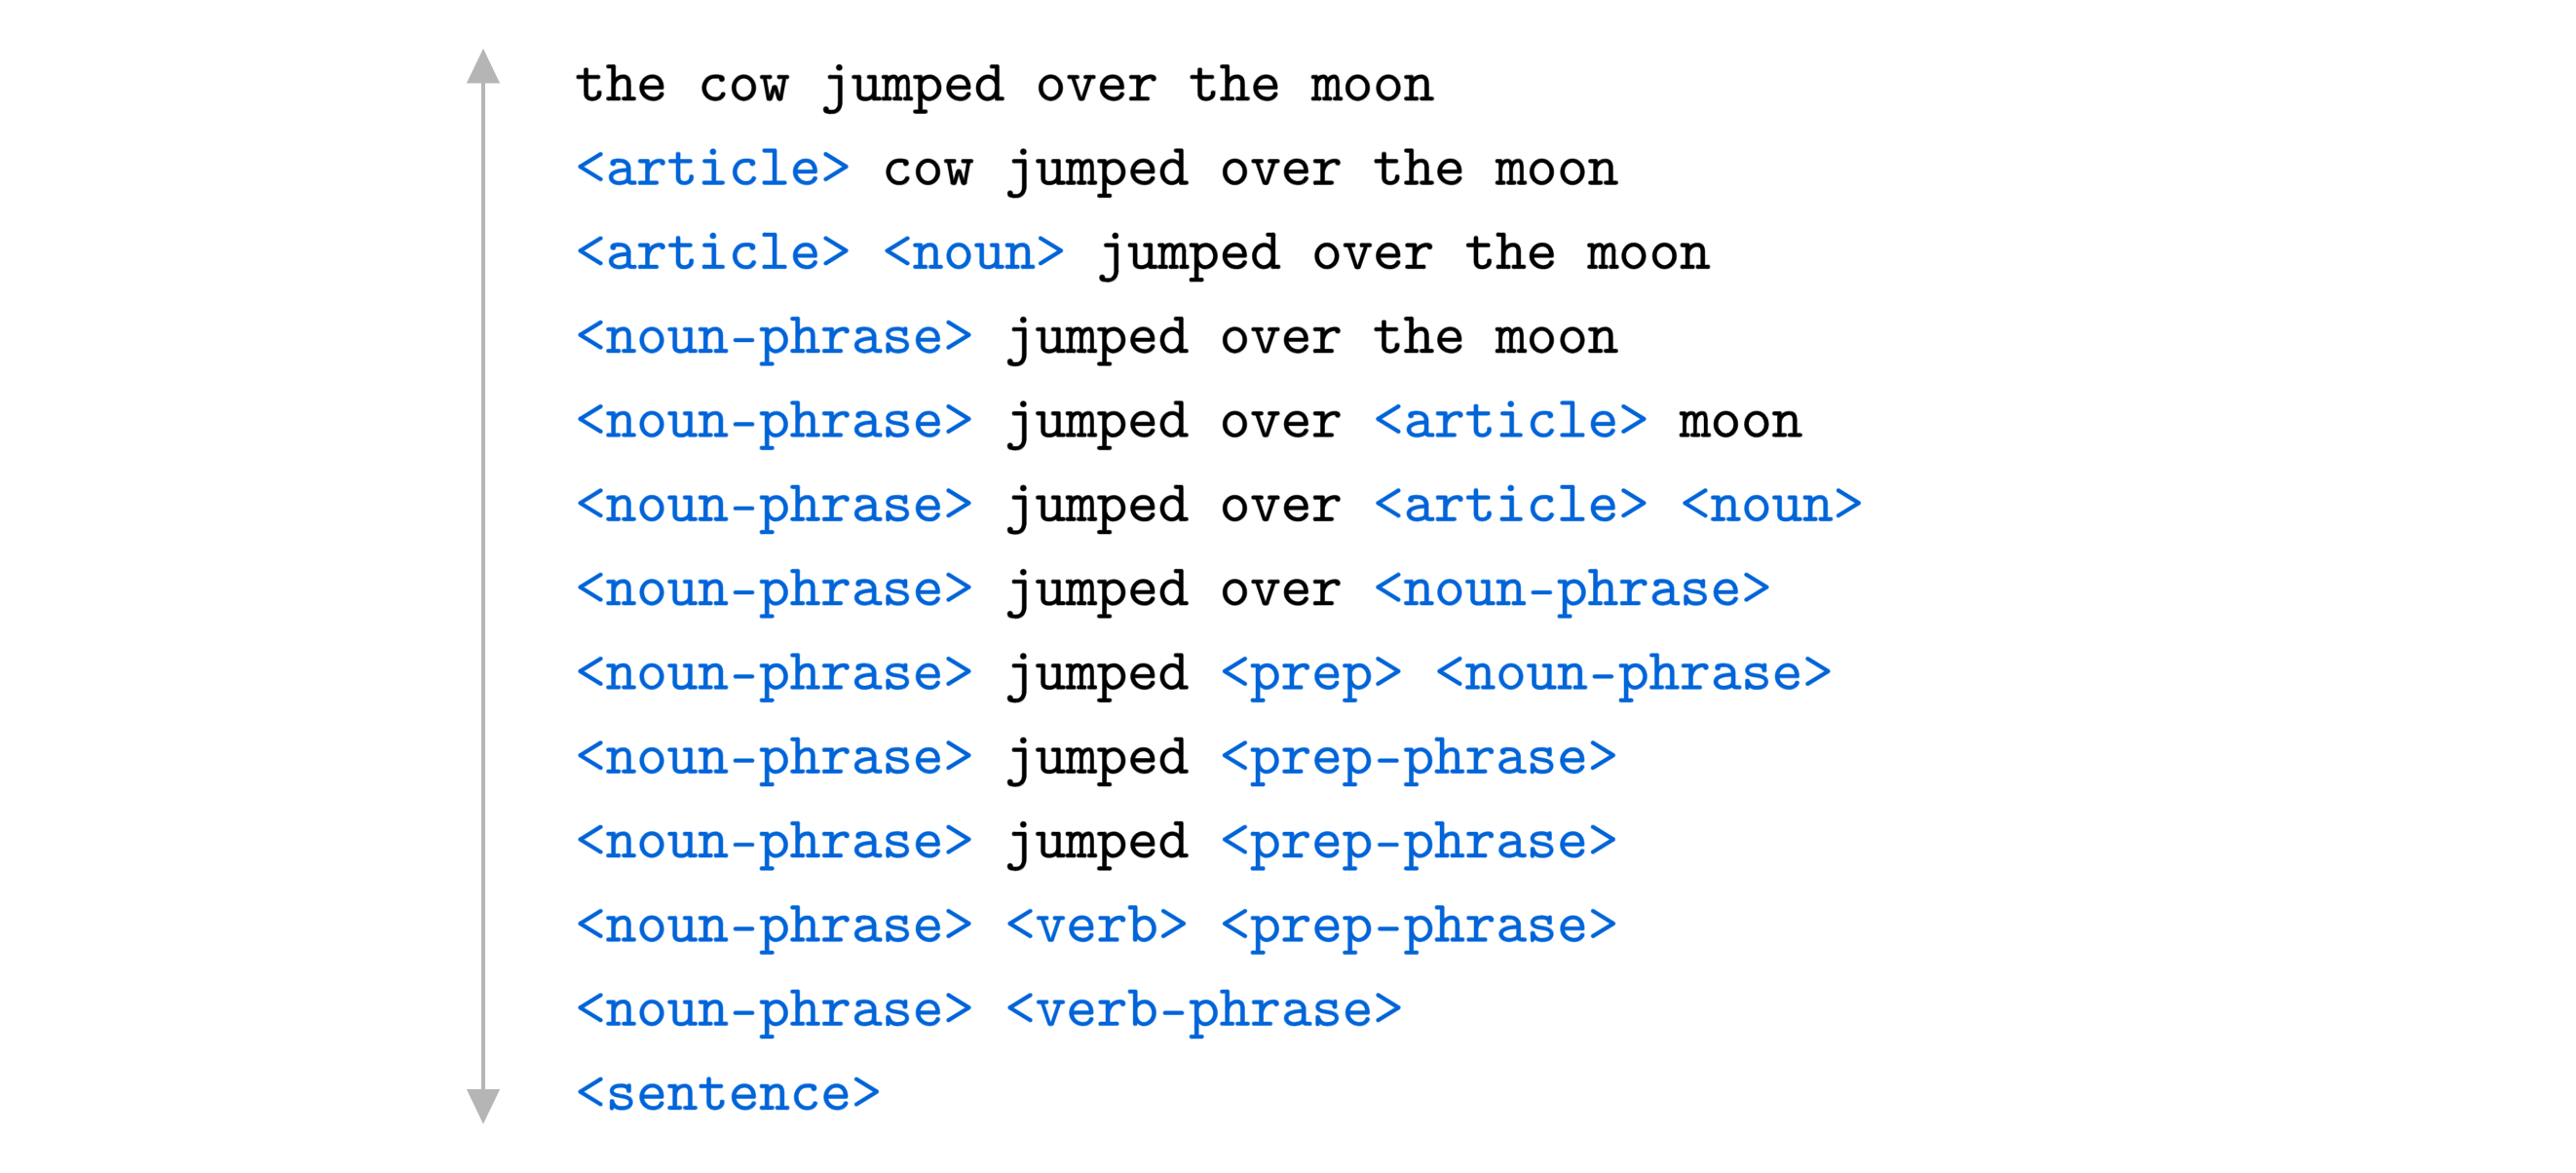
\includegraphics[width=1\textwidth]{Sections/Formal/derivation.png}
    \caption{The sentence ``The cow jumped over the moon.'' broken down into terminal and non-terminal symbols. This is a derivation showing how the sentence is built up from the start symbol of a \texttt{<sentence>}.}
\end{figure}

\noindent
From which the above can be represented in a tree structure:
\begin{figure}[h]
    \centering
    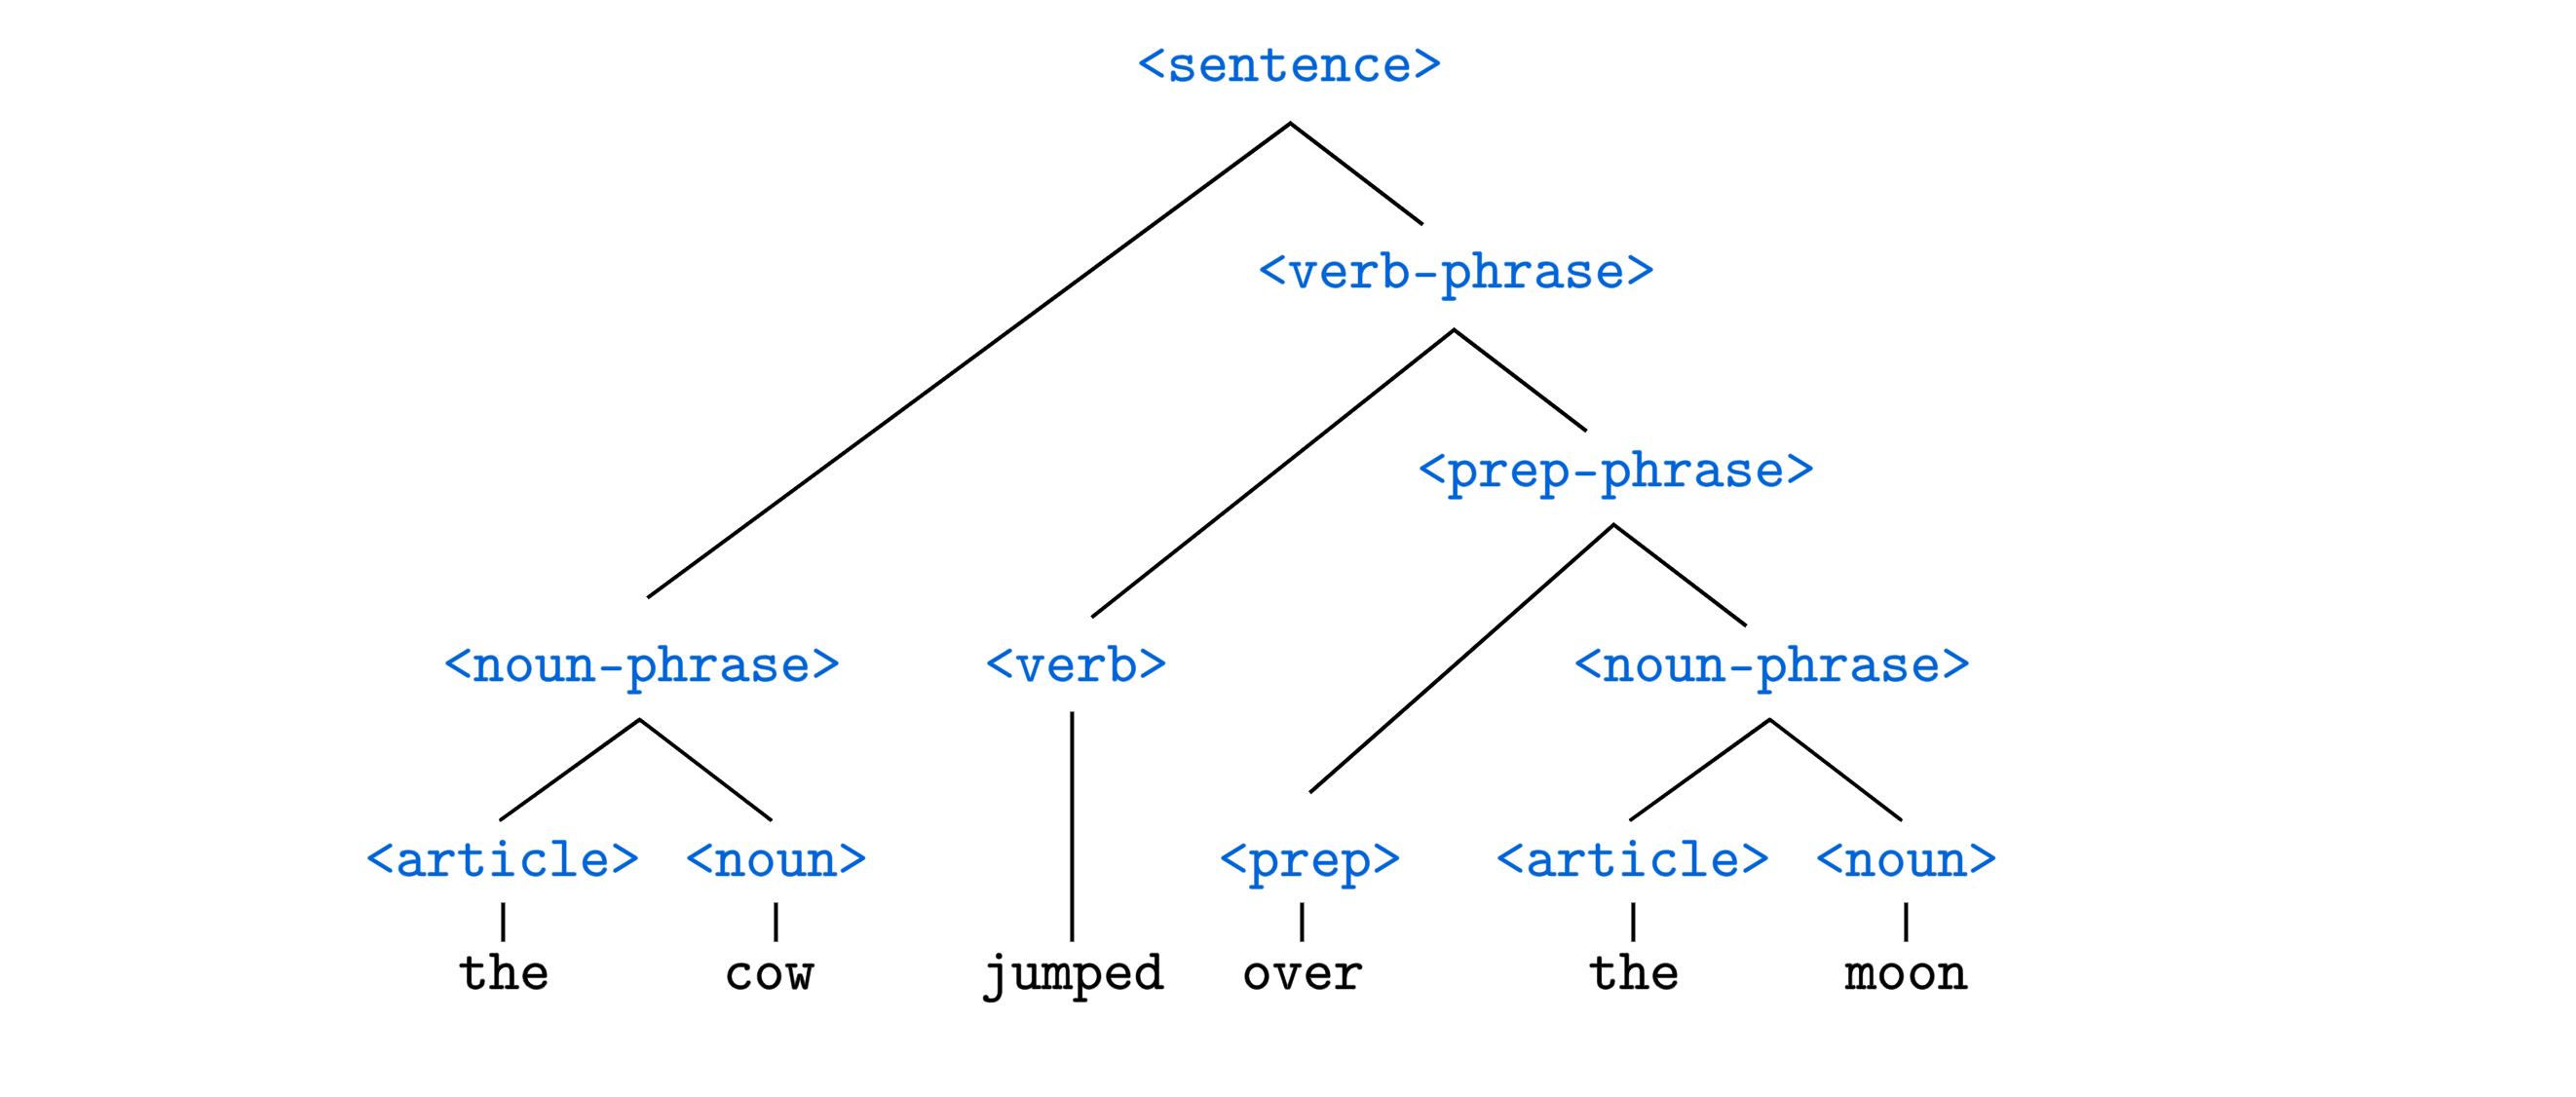
\includegraphics[width=1\textwidth]{Sections/Formal/tree.png}
    \caption{The sentence ``The cow jumped over the moon.'' represented as a \textbf{parse-tree}.}
\end{figure}

\newpage

\noindent
Now if we wanted to state these rules before-hand that a \texttt{<sentence>} is made up of a \texttt{<noun-phrase>} and a \texttt{<verb-phrase>} we can do so as such:

\begin{figure}[h]
    \centering
    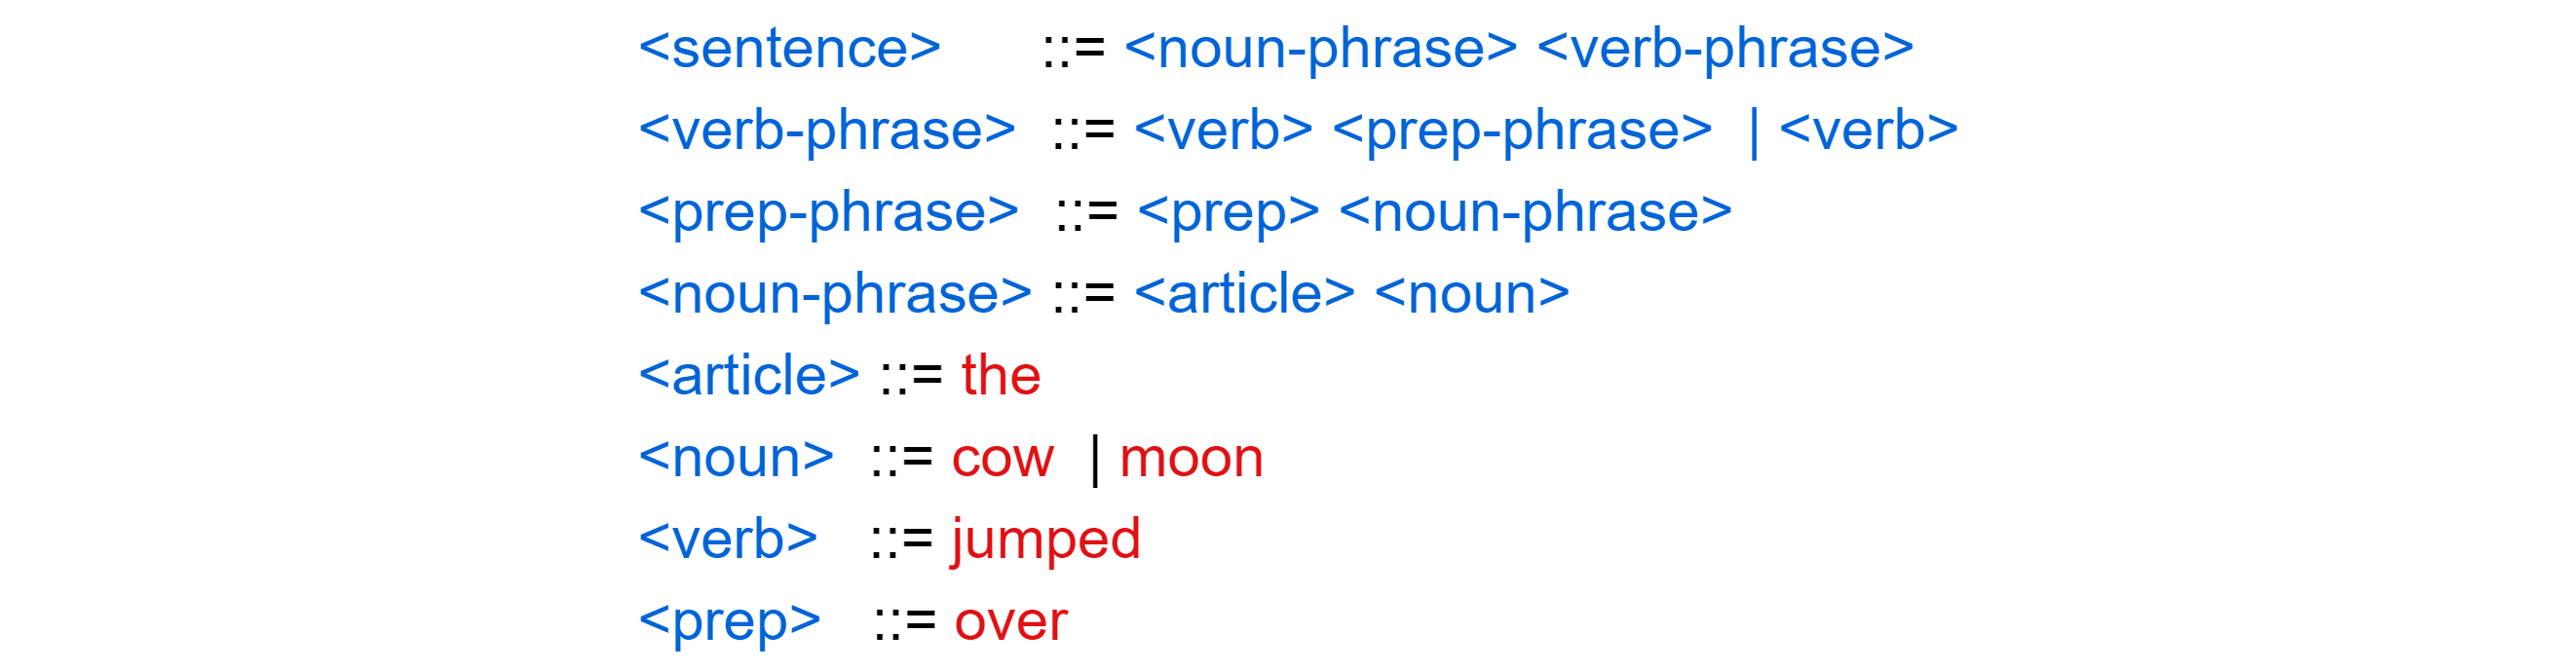
\includegraphics[width=1\textwidth]{Sections/Formal/bnf.png}
    \caption{The rules for the sentence ``The cow jumped over the moon.'' via a thread of production rules (\ref{def:production_rule}). This example illustrates \textbf{Backus-Naur Form (BNF)} notation.}
\end{figure}

\vspace{-1em}
\begin{Def}[Backus-Naur Form (BNF)]

    \textbf{Backus-Naur Form (BNF)} is a formal notation used to define the context. It consists of production rules that specify how symbols in a language can be recursively composed. Each rule follows the form:
    
    \begin{center}
    \texttt{<non-terminal> ::= expression}
    \end{center}
    
    \noindent
    where \texttt{<non-terminal>} represents a syntactic category, and \texttt{expression} consists of terminals, non-terminals, or alternative sequences.
    
    \end{Def}

    \vspace{-.5em}
    \noindent
        Consider a more programmer-like example, assuming we read from left-to-right:

        \begin{figure}[h]
            \centering
            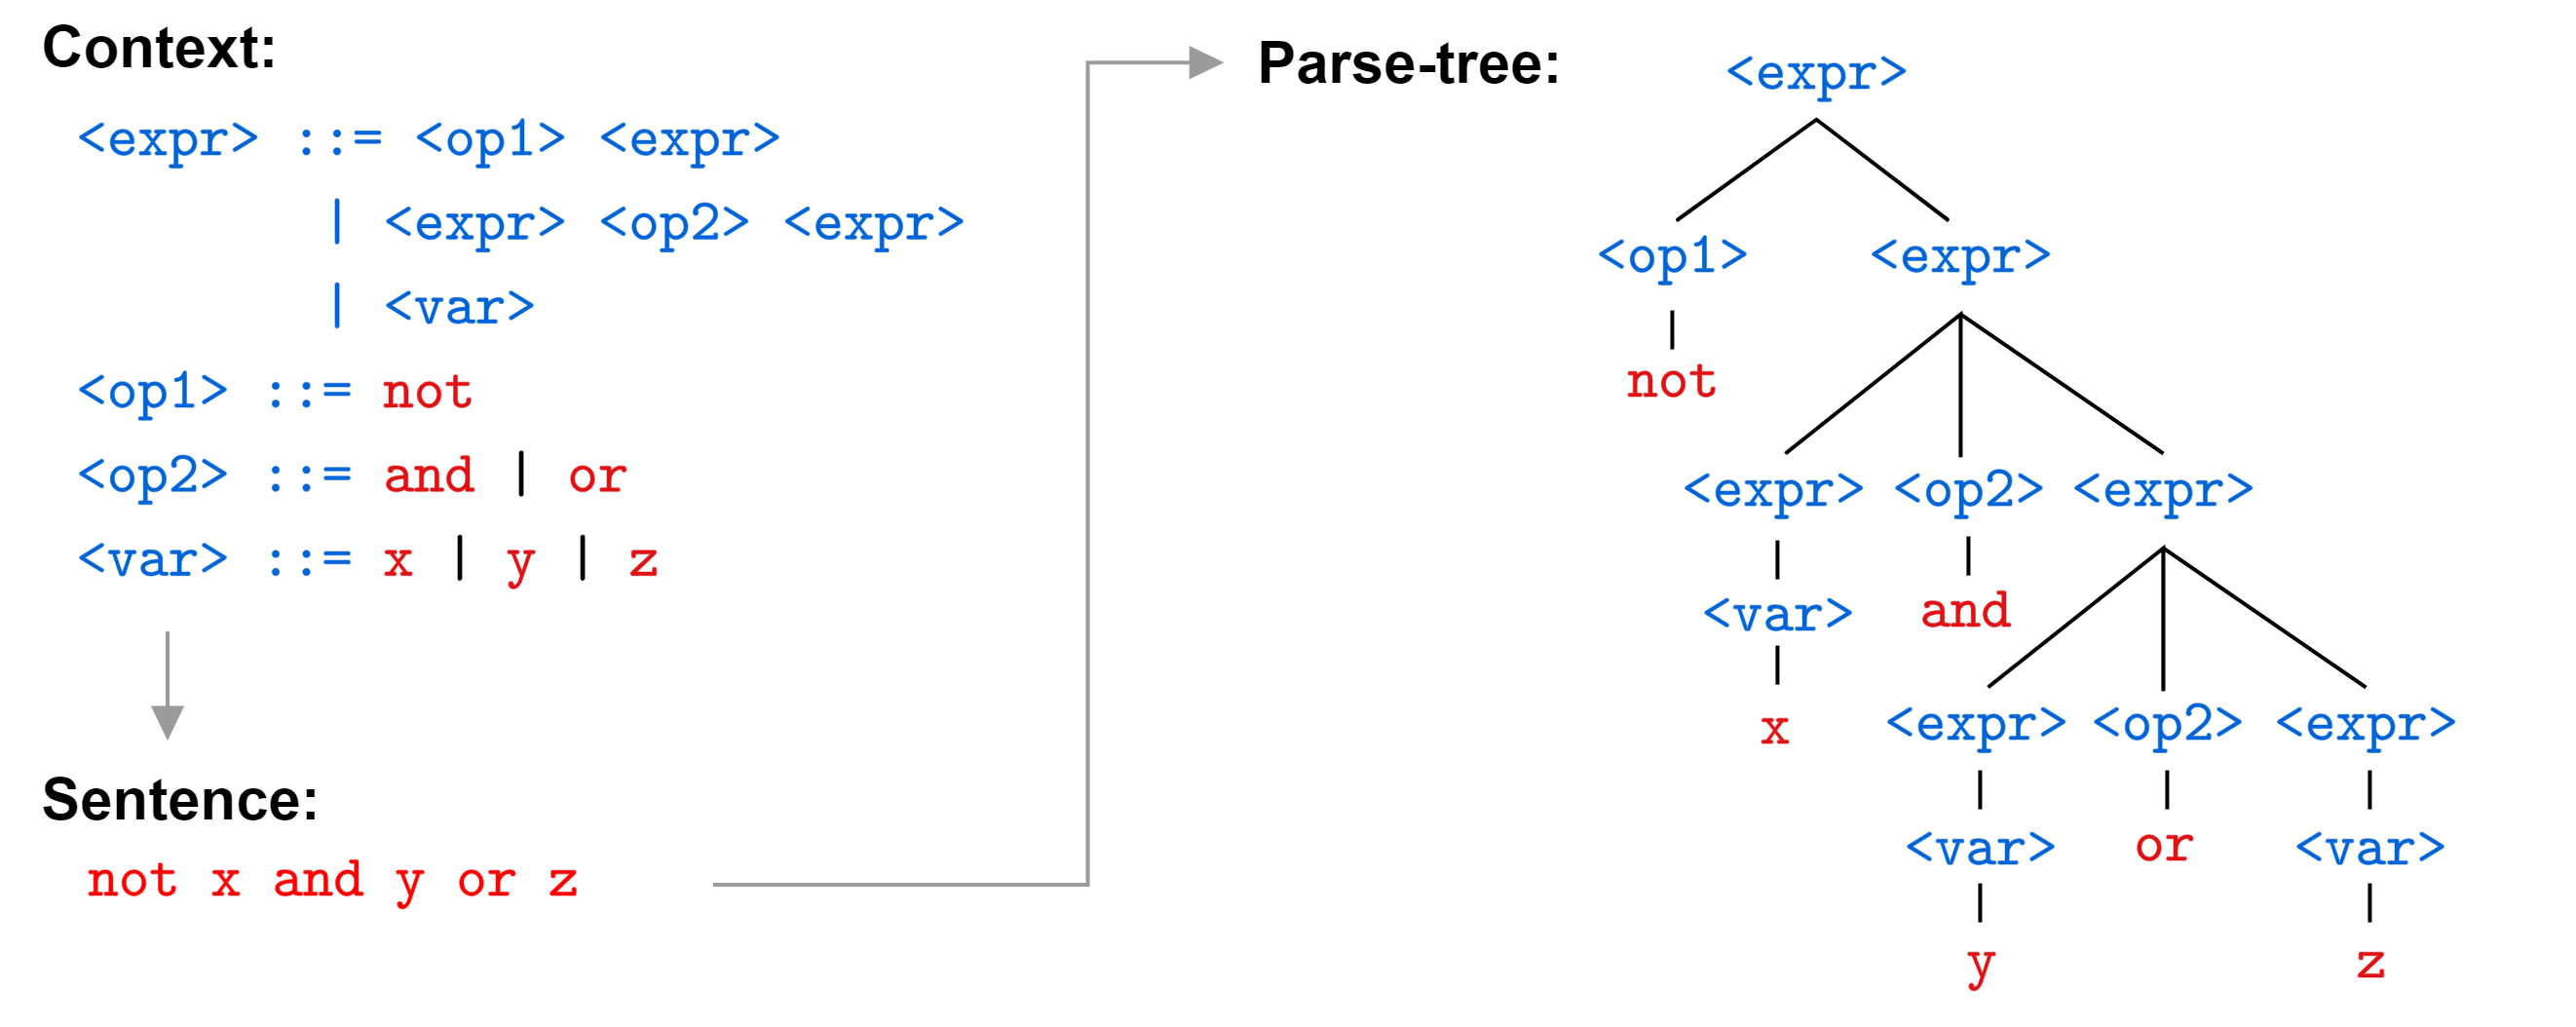
\includegraphics[width=1\textwidth]{Sections/Formal/bnf2.png}
            \caption{A simple language, consisting of \texttt{and} and \texttt{or} operations.}
            \label{fig:bnf2}
        \end{figure}

\newpage

\noindent
The process of taking non-terminal symbols and replacing them with terminal symbols is called a \textbf{leftmost derivation}.
\begin{Def}[Leftmost Derivation]

    A \textbf{leftmost derivation} is a sequence of sentential forms in which, at each step, the \textbf{leftmost} non-terminal symbol is replaced according to a production rule. This process continues until the entire string consists only of terminal symbols. Leftmost derivations are useful for defining deterministic parsing strategies and constructing parse trees in a structured manner.
    
\end{Def}
    
\subsection{Ambiguity in Grammars}

In natural language we have cases where what we say can be ambiguous. For example,
\begin{center}
    \textit
    {``The duck is ready for the dinner table.''}
\end{center}

\noindent
Natural questions may arise:
\begin{itemize}
    \item Was the duck ready to be eaten?
    \item Was the duck preparing the table for dinner?
    \item Was the duck a wrestler, ready to body-slam a constituent?
\end{itemize}
\noindent
For instance, let's clean up the previous sentence, avoiding any and all ambiguity:
\begin{center}
    \textit
    {``The duck is ready \textbf{to body slam} the dinner table.''}
\end{center}
\noindent
Now Consider the previous example of \texttt{and} and \texttt{or} operations from Figure (\ref{fig:bnf2}):
\begin{figure}[h]
    \centering
    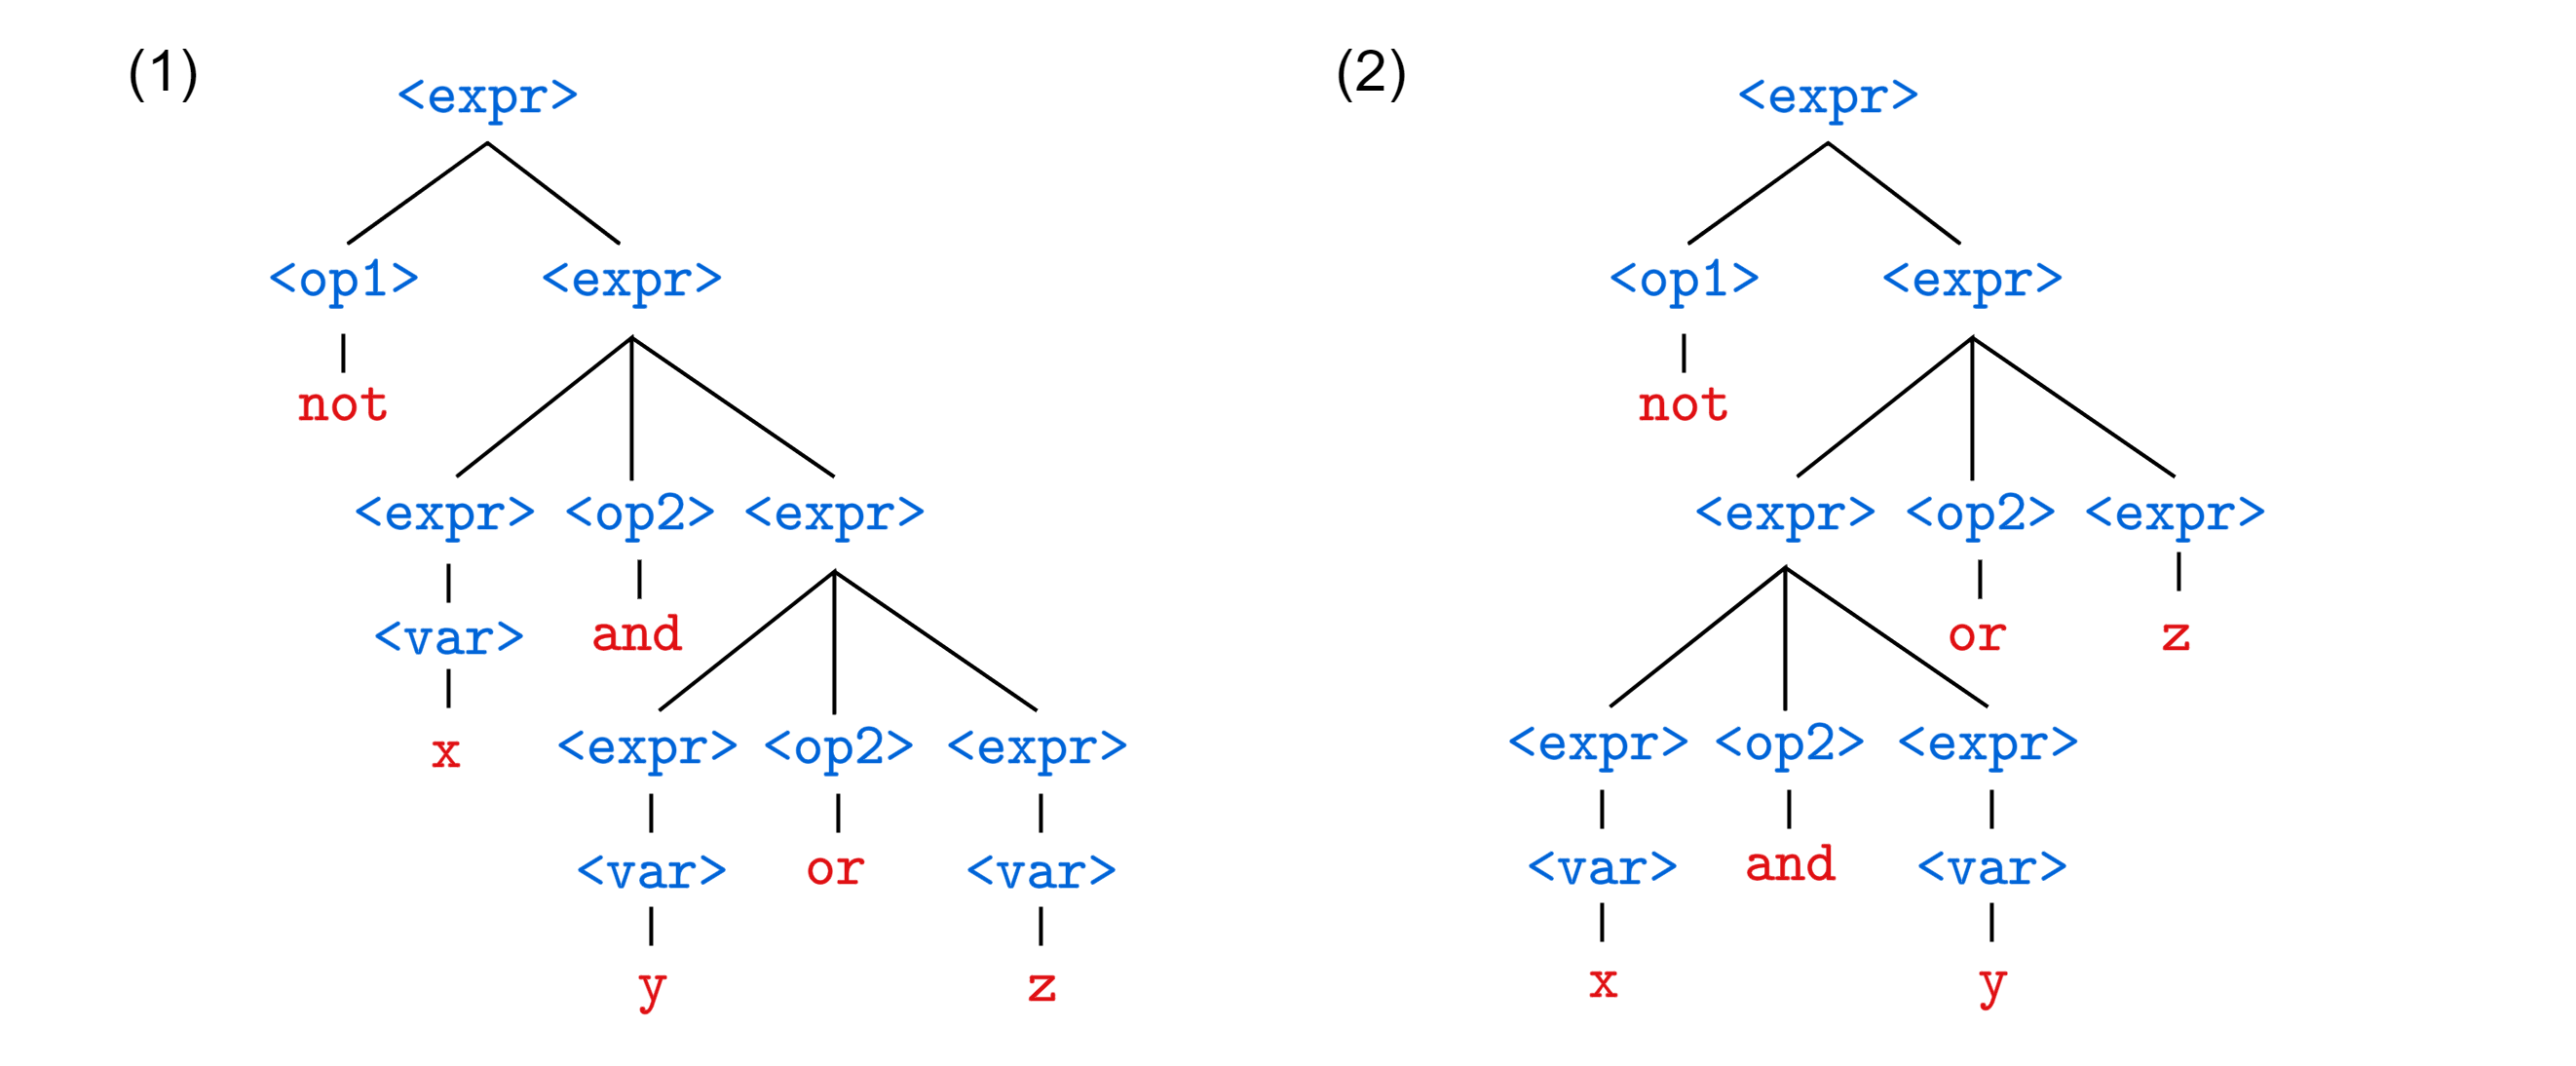
\includegraphics[width=1\textwidth]{Sections/Formal/amb.png}
    \caption{Two possible parse-tree derivations based off of Figure (\ref{fig:bnf2}). (1) Shows our previous intention, while (2) shows a different interpretation, if parsing order was not specified.}
    \label{fig:amb}
\end{figure}

\newpage

\noindent
In Figure (\ref{fig:amb}), (1) shows, \texttt{\textcolor{Wine}{not x and (y or z)}} while (2) shows, \texttt{\textcolor{Wine}{not (x and y) or z}}. This ambiguity can cause issues; for example, 
$x=y=False$, $z=True$, yields different results for (1) and (2). \\

\begin{Def}[Ambiguity in BNF Grammar]

    A \textbf{BNF grammar} is \textbf{ambiguous} if there exists a sentence with multiple valid parse-trees.
\end{Def}
    
\noindent
These, small pieces of ambiguity can crop up anywhere. Consider the following example:
\begin{figure}[h]
    \centering
    
\includegraphics[width=1\textwidth]{Sections/Formal/amb2.png}
    \caption{An ambiguous grammar \texttt{if} expressions.}
    \label{fig:amb2}
\end{figure}

\noindent
In Figure (\ref{fig:amb2}), contains sub-cases which can lead to ambiguity. As, ``is it the sub-case or the super-case?'' For 
example, consider:
\begin{center}
    \texttt{\textcolor{Wine}{if x then (if y then z else w)}} or is it \texttt{\textcolor{Wine}{if x then (if y then z) else w}}
\end{center}

\noindent 
These problems often arise when interpreting expressions at the linear level. On an important note:
\begin{theo}[Ambiguity is Undecidable]
    
    It is impossible to write a generalized program to determine if a given grammar set is ambiguous.
    This requires to finding all possible sentences; \textbf{However}---our grammar is recursive---this would mean generating 
    an infinite number of sentences.
\end{theo}

\noindent
Though we can avoid ambiguity by specifying our operation order:
\begin{Def}[Fixity]

    The \textbf{fixity} of an operator refers to its placement relative to its operands:
    
    \begin{itemize}
        \item \textbf{Prefix}: The operator appears \textit{before} its operand (e.g., $f\ x$, $-x$).
        \item \textbf{Postfix}: The operator appears \textit{after} its operand (e.g., $a!$ for factorial or dereferencing).
        \item \textbf{Infix}: The operator appears \textit{between} two operands (e.g., $a * b$, $a + b$, $a \mod b$).
        \item \textbf{Mixfix}: The operator is interleaved with its operands, appearing in multiple positions (e.g., \texttt{if} $b$ \texttt{then} $x$ \texttt{else} $y$).
    \end{itemize} 
    \end{Def}

\newpage 
\noindent
So by specifying only Prefix or only Postfix operations ambiguity can be avoided:
\begin{Def}[Polish Notation]

    \textbf{Polish Notation} is a notation for arithmetic expressions in which the operator precedes its operands. For example, the polish notation $- / + 2 * 1 - 2 3$ is written as $- (2 + (1 * (- 2) / 3)$.\\
    
    \noindent
    In contrast, \textbf{Reverse Polish Notation} (RPN) places the operator after its operands. For example, Infix: $(3 + 4) * 5$ is $3\ 4 + 5\ *$ in RPN.
\end{Def}

However, this is not always practical. Consider \texttt{if} expressions dealt this way:
\begin{figure}[h]
    \centering
    
\includegraphics[width=1\textwidth]{Sections/Formal/amb3.png}
    \caption{An unambiguous grammar for \texttt{if} expressions.}
    \label{fig:amb3}
\end{figure}

\noindent
Likewise, if we decided to enforce parenthesis everywhere it might be a bit cumbersome:
\begin{figure}[h]
    \centering
    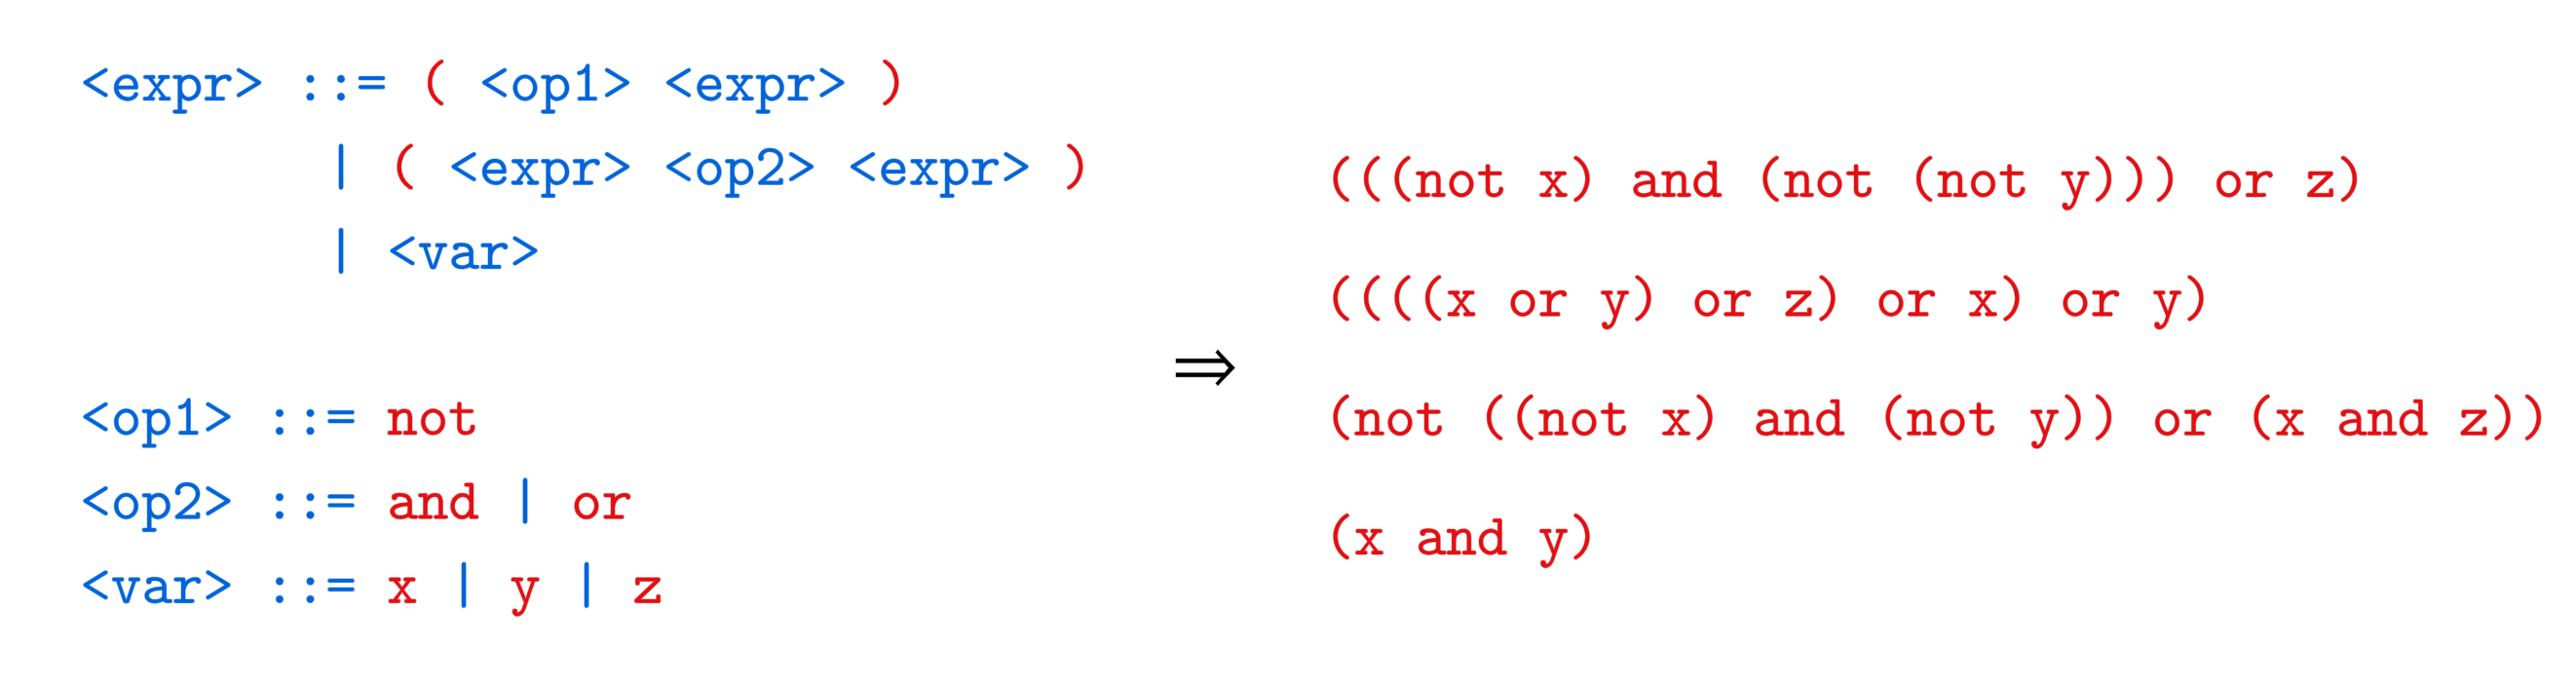
\includegraphics[width=1\textwidth]{Sections/Formal/amb4.png}
    \caption{An unambiguous grammar for \texttt{and or not} expressions, with parenthesis everywhere.}
    \label{fig:amb4}
\end{figure}

\noindent
\begin{theo}[The Ambiguity of Associativity \& Precidence Rules]
    
    \begin{itemize}
        \item \textbf{Associativity}: $a + b + c$ is ambiguous, as it could be $(a + b) + c$ or $a + (b + c)$.
        \item \textbf{Precedence}: $a + b * c + d$ is ambiguous, as it could be $(a + (b * c)) + d$ or $a + ((b * c) + d)$.
    \end{itemize}
    \end{theo}
\newpage 

\noindent
We can resolve this by breaking the symmetry of our grammar:
\begin{theo}[Resolving Associativity: Breaking Symmetry]

    The reason for ambiguity often comes symmetry in grammar rules of form:
    \begin{center}
        \texttt{<expr> ::= <expr> <op> <expr>}\\
        \texttt{<op> ::= + | - | ...} \hspace{1.8em} \null
    \end{center}

    \noindent
    This means that the left or right side can be expanded indefinitely. By breaking this symmetry, we can resolve ambiguity:
    \begin{center}
        \texttt{<expr> ::= <var> <op> <expr>}\\
        \texttt{<op> ::= + | - | ...} \hspace{1.3em} \null\\
        \texttt{<var> ::= x | y | z | ...} \hspace{-.3em} \null
    \end{center}
    \noindent
    In the above we fixed the left side to be a \texttt{<var>} and the right side to be an \texttt{<expr>}.
    This makes our expression \textbf{right-associative}. Vice-versa, if we fixed the right side, it would be \textbf{left-associative}.
\end{theo}

\begin{theo}[Resolving Precedence: Factor Out Higher Precedence]

    Precedence issues arise when operations reside on the same level. For instance,
        
    \vspace{-1em}
        \begin{align*}
            \texttt{<expr>} &\texttt{::= <expr> + <expr> | <expr> * <expr>}
        \end{align*}

    \noindent
    Here, it's unclear whether \texttt{+} or \texttt{-} should be evaluated first. By factoring out higher precedence operations, we can resolve this, 
    as, \underline{\textbf{terms deeper in the parse tree are evaluated first}}:
    \begin{align*}
        \texttt{<expr>} &\texttt{::= <expr> + <term> | <term> }\\
        \texttt{<term>} &\texttt{::= <term> * <var> | <var>}\\
        \texttt{<var>} &\texttt{::= x | y | z | ...}
    \end{align*}

    \vspace{-1em}
    \noindent
    Here, \texttt{*} has higher precedence than \texttt{+}, as it's deeper in the parse tree. To handle 
    \textbf{parentheses}, we can introduce another factor:
    \begin{align*}
        \texttt{<expr>} &\texttt{::= <expr> + <term> | <term> }\\
        \texttt{<term>} &\texttt{::= <term> * <var> | <pars>}\\
        \texttt{<pars>} &\texttt{::= var | ( <expr> )}\\
        \texttt{<var>} &\texttt{::= x | y | z | ...}
    \end{align*}
    \noindent
    Intuitively, in expressions like \texttt{(a + b) * c}, we want to treat \texttt{(a + b)} as a single unit/\textit{variable}. \textbf{Note},
    the parentheses are tokens surrounding the non-terminal \texttt{<expr>}.
\end{theo}

\newpage 

\noindent
Now consider the \texttt{and or not} expressions from Figure (\ref{fig:bnf2}) resolving the associative ambiguity:

\begin{figure}[h]
    \centering
    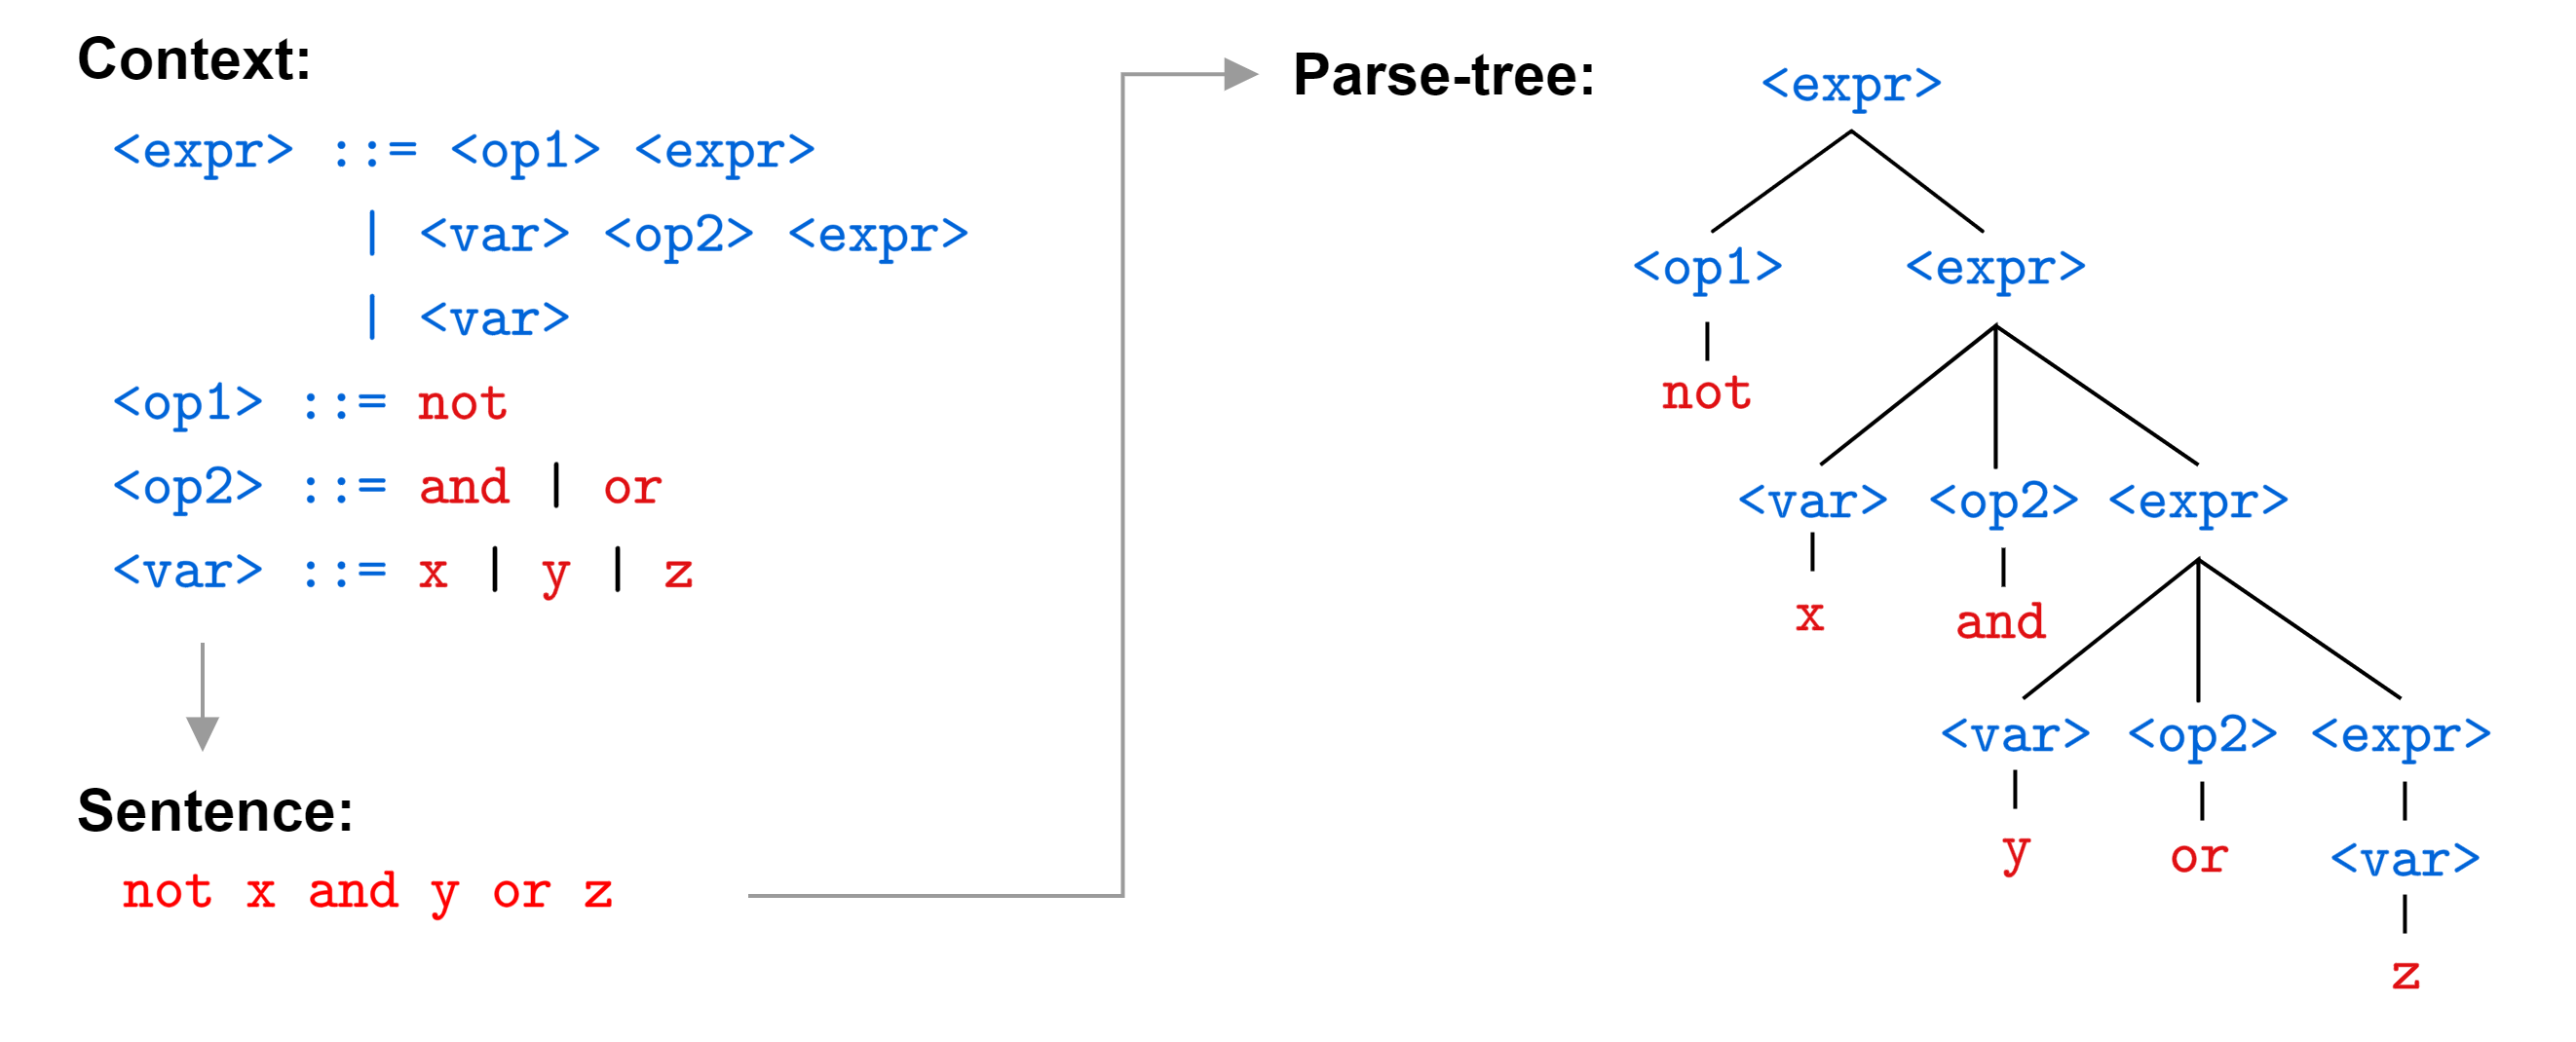
\includegraphics[width=1\textwidth]{Sections/Formal/amb5.png}
    \caption{An unambiguous grammar for \texttt{and or not} expressions, by breaking symmetry.}
    \label{fig:amb5}
\end{figure}

\noindent
Now we put all the rules together:
\begin{figure}[h]
    \centering
    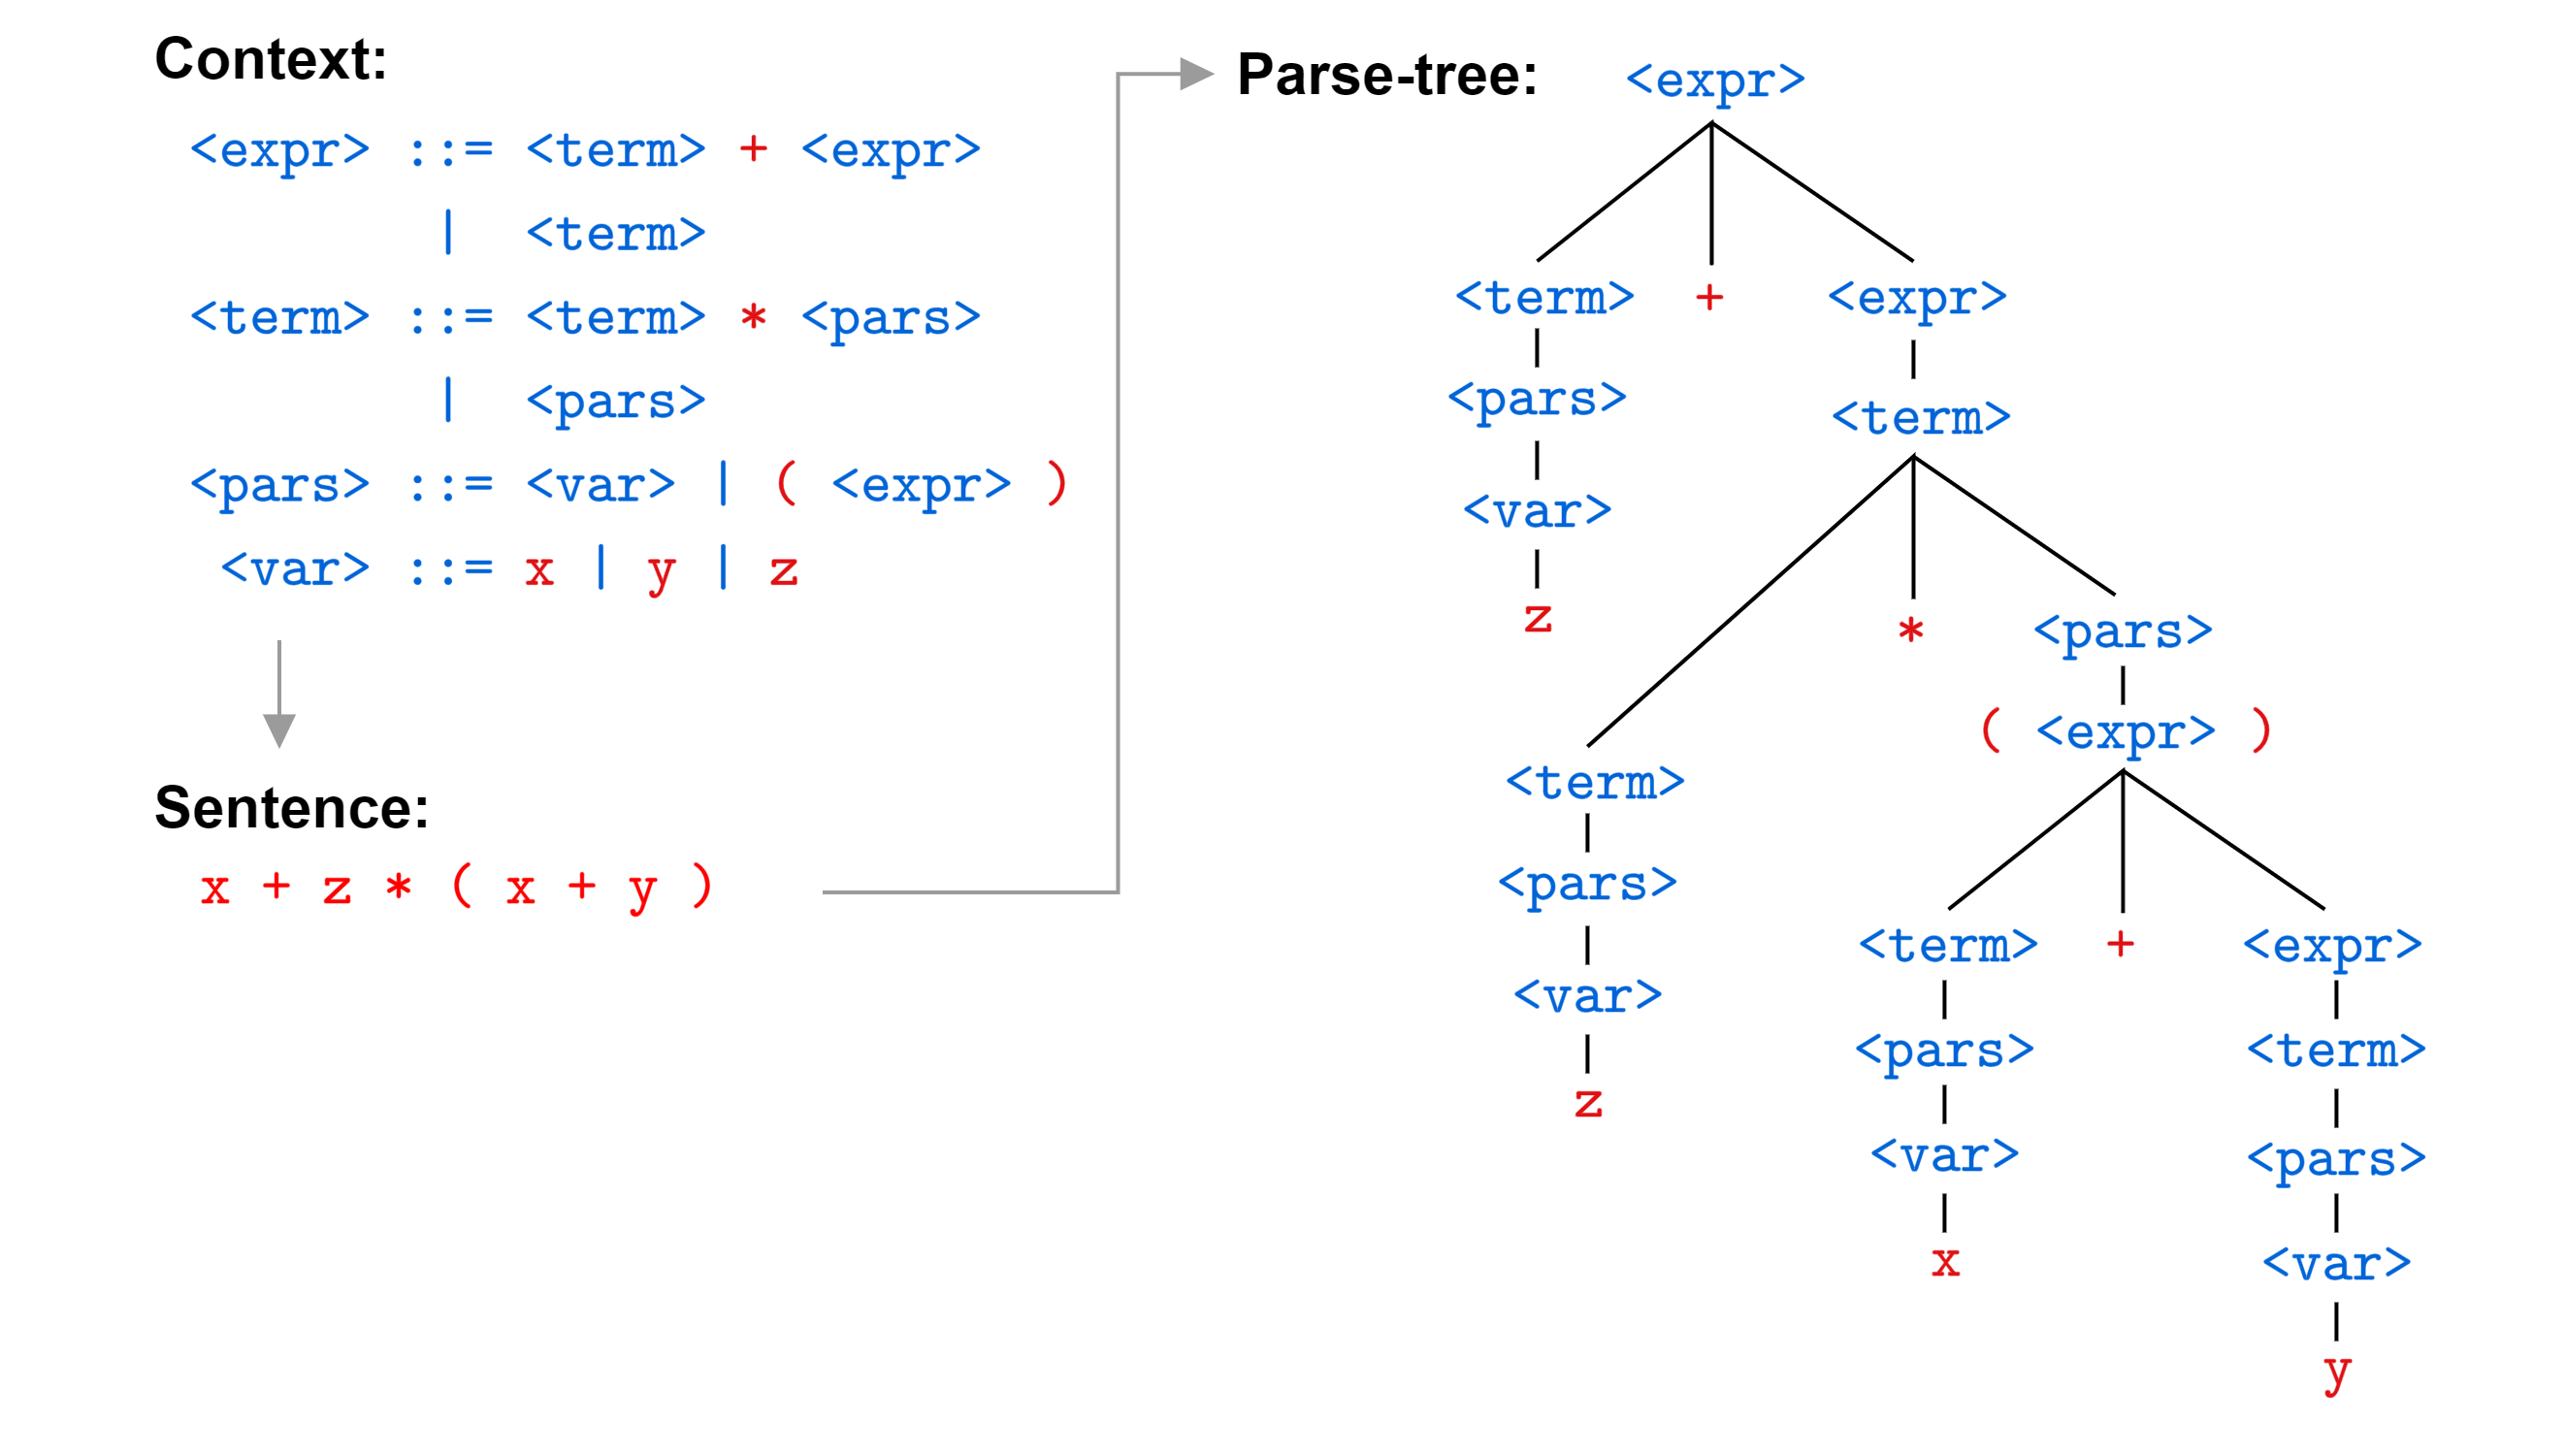
\includegraphics[width=1\textwidth]{Sections/Formal/amb6.png}
    \caption{An unambiguous grammar for \texttt{+, *} expressions, by breaking symmetry and precedence.}
    \label{fig:amb6}
\end{figure}

\begin{Tip} \textbf{The ``Cult of Parentheses" in Lisp:} Lisp-style languages rely heavily on \textbf{prefix notation}, where operators and function names appear \textbf{before} their arguments. This leads to deeply nested \textbf{parentheses}, often making Lisp code look overwhelming to newcomers.\\
    
    \noindent
    For example, the Fibonacci function in Lisp is written as:
    
    \begin{lstlisting}[numbers=none]
    (defun fib (n)
      "Return the nth Fibonacci number."
      (if (< n 2)
          n
          (+ (fib (- n 1))
             (fib (- n 2)))))
    \end{lstlisting}
    
    \noindent
    Since \textbf{everything} in Lisp is an expression and follows a \textbf{uniform syntax}, parentheses are required for every function call, condition, and operation. This often leads to \textbf{excessive nesting}, and the title, \textbf{``Cult of Parentheses"}.
    
    \end{Tip}
    
    